\section{Stage 4: IDE Extension} \label{sec:work_stage4_extension_build}

{\color{blue}The last component is the extension for an IDE, capable of predicting energy consumption. 
To provide this insight to developers it is necessary to build a tool that can provide all of that. Integrating the tool into an IDE makes it easier to understand and use, which are some of our main goals. With this the developer only needs to download an extension for an IDE and will access to the insights provided by the tool.

In this project, we choose the VSCode due to its lightweight architecture, extensive community support, and ease of extension development using familiar web technologies such as JavaScript and TypeScript. This extension allows the user to have a better understanding of how much energy the code is consuming, and what are the methods, and variables that most affect it.

It is important to note that the extension tool will serve as a guide, providing energy consumption estimates to raise awareness rather than dictate action. Ultimately, it is up to developers to decide whether to prioritize performance, energy efficiency or any other factor. For example, if a program only needs to run within a certain timeframe and can afford a slight reduction in performance, developers may choose to trade some performance for improved energy efficiency, making more informed decisions thanks to the insights provided by the tool.

To ensure efficiency, the tool uses static analysis to parse the code into an AST. From the AST, it analyzes the code and, using previously collected models, estimates the energy cost of the operations.}


When opening the extension side page, it contains sliders that can change the input values, and it has the estimate button, to predict the energy.

The extension analyzes the user's Java files, identifies all the methods used, and matches them against a set of pre-trained models. Then it finds which variables affect those methods, meaning the variables that are the inputs to the method. For example, in \texttt{list.add(i)}, the relevant inputs and variables are \texttt{list} and \texttt{i}. The variable \texttt{list} is important because its size may impact energy consumption, while \texttt{i} is a method input whose different values can lead to varying method behavior, which can also impact the energy consumption.
The extension does this to every method it finds in the source code and groups it by method. In the end it creates groups of input variables for each method, displaying it in sliders. The sliders allow the user to change the input values and when pressing the estimate button and, based on the values, it will change the energy estimation.

If a method calls another user-defined method that already has an assigned energy cost (but was not used to train the machine learning models), then the calling method will also include that energy cost. This part was done by first analyzing individual methods for the model-trained methods and get their base energy. In a second iteration, each method is traversed to determine which calls are made, how many calls are made, and whether the calls are inside or outside loops. With this information, the total energy cost of each method could be calculated, accounting for both direct and indirect calls to model-trained methods.

When a model-trained method or a user-defined method are called inside a loop, a new slider appears to represent the loop size. The method’s energy cost is multiplied by this loop size. In the case of nested loops, the energy cost is multiplied by the product of all nested loop sizes. Note that only methods and variables that affect the energy appear on the panel.

This extension can help understand how much energy the code is using.
For example, the snippet in listing~\ref{lst:Java_program_to_count_word_frequencies_in_a_string} counts how many times each word appears in a given text string, can be estimated for how much energy it uses.

\begin{listing}[htbp]
\noindent\rule{\linewidth}{0.4pt}
\begin{minted}[linenos, fontsize=\small, frame=none, bgcolor=white,breaklines=true,breakanywhere=true]{Java}
    public class WordFrequency {
    public static HashMap<String, Integer> countWordFrequency(String text) {
        String[] words = text.toLowerCase().split("\\W+");
        HashMap<String, Integer> frequencyMap = new HashMap<>();
        for (String word : words) {
            if (word.isEmpty()) continue; 
            String temp = frequencyMap.getOrDefault(word, 0) + 1;
            frequencyMap.put(word, temp);
        }
        return frequencyMap;
    }
    public static void main(String[] args) {
        String input = "Java is simple. Java is powerful.";
        HashMap<String, Integer> result = countWordFrequency(input);
        System.out.println(result);
    }
}
\end{minted}
\noindent\rule{\linewidth}{0.4pt}
\caption{Java program to count word frequencies in a string}            
\label{lst:Java_program_to_count_word_frequencies_in_a_string}
\end{listing}

Figure~\ref{fig:extension_example1} illustrates how the extension displays the energy consumption of the code in Listing~\ref{lst:Java_program_to_count_word_frequencies_in_a_string}. In the figure two methods \texttt{countWordFrequency(String)} and \texttt{main(String[])} can be seen, next to their energy consumption estimations. Its also shown under the box with the method's name, the important variables that can affect energy consumption. For instance, in the method \texttt{countWordFrequency(String)} it can be seen that the size of the variables \texttt{word} and \texttt{frequencyMap} can change the energy usage. Also, the loop size is taken into account, and the number operations performed will impact the energy significantly.

{\color{blue}When calling the method \texttt{Map.put(Object, Object)}, the extension tool shows more options available in the slider menu. The Figure~\ref{fig:extension_example1}, illustrates the variables that appear when the method is used. It is noticeable that four sliders are available to change, and they contain the three variables used in the method \texttt{frequencyMap.put(word, temp)}. The first one is the collection input, \texttt{frequencyMap}, the second input is the String variable \texttt{word}, and the last input is the String variable \texttt{temp}. All these three variables were detected by the extension tool and marked as important. The last slider that is displayed in the image is the loop, which can also affect the energy output, so it is also marked as important by the extension tool.}



\begin{figure}[htbp]
  \centering
  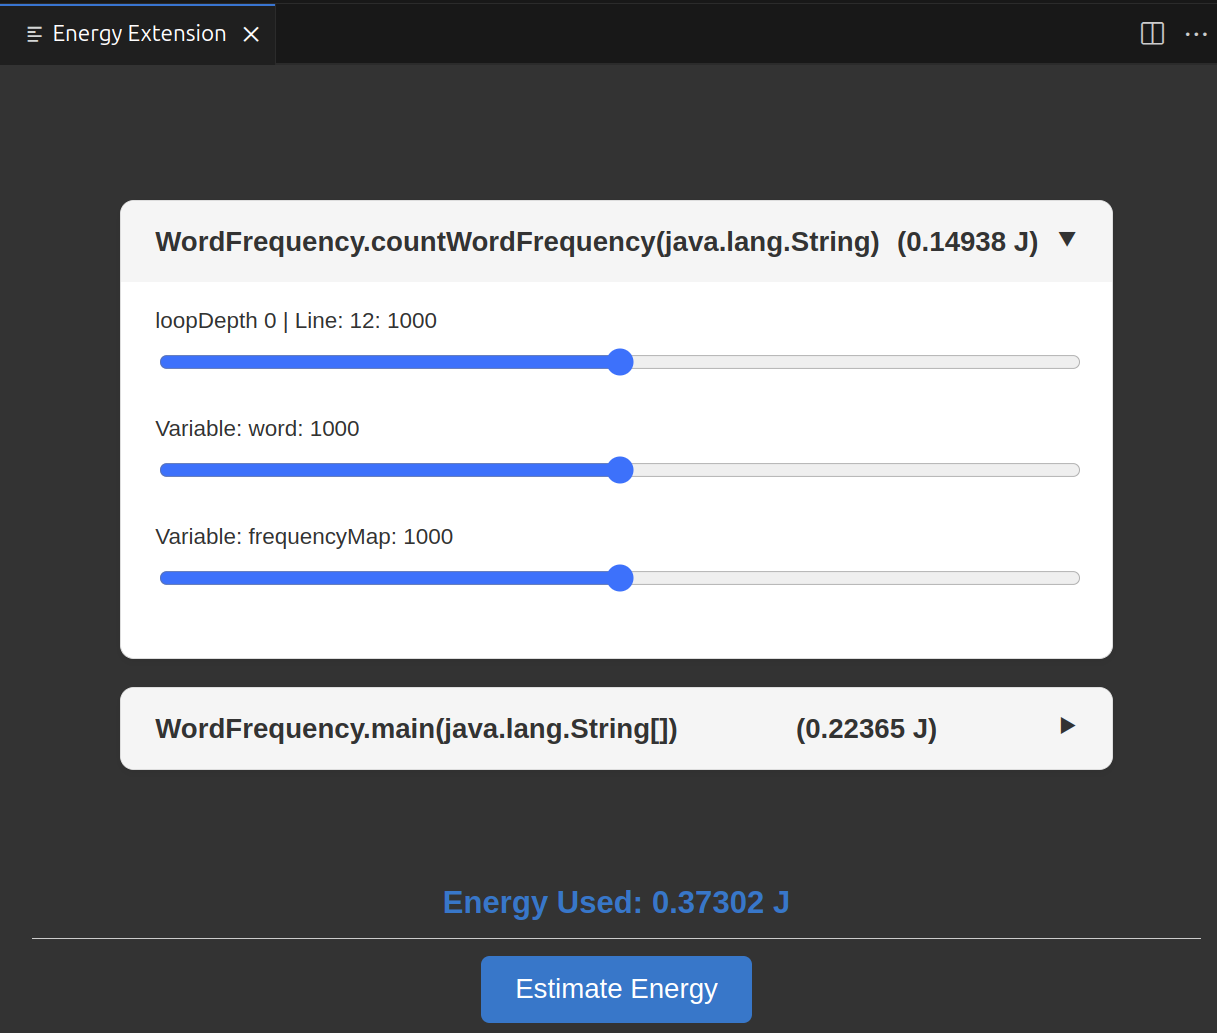
\includegraphics[width = .7 \textwidth]{figures/extension_example1.png}
  \caption{Extension example HashMap}
  \label{fig:extension_example1}
\end{figure}


Another example can be see in the Figure~\ref{fig:extension_example2}, where the same code is used, but instead of using a \texttt{HashMap} it uses a \texttt{TreeMap}. The energy consumption is different, as the model was trained to understand that the \texttt{TreeMap} consumes more energy than the \texttt{HashMap}.

%If, for instance, instead of using \texttt{HashMap}, \texttt{TreeMap} is used, the energy differences can easily be noticed in the Figure~\ref{fig:extension_example2}. This shows a great example of how two implementations of the same collection can differ in energy. It can also be used to compare different method implementations, that achieve the same output but rely on different approaches.



\begin{figure}[htbp]
  \centering
  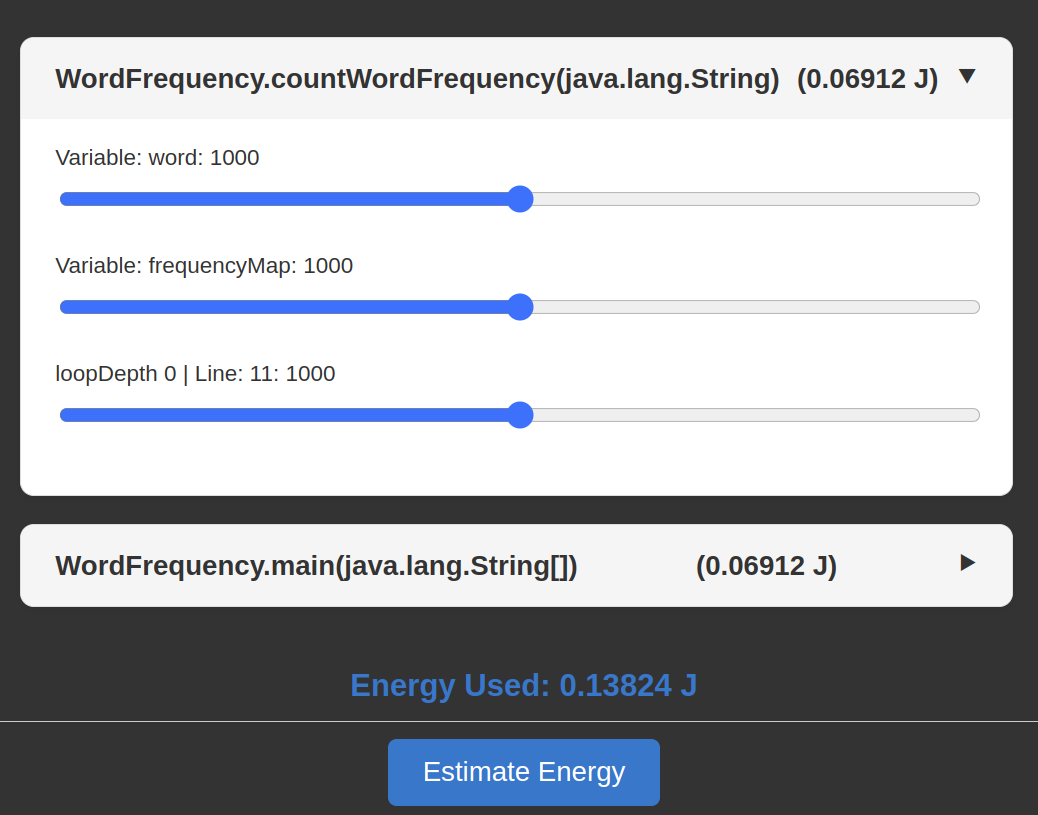
\includegraphics[width = .7 \textwidth]{figures/extension_example2.png}
  \caption{Extension example TreeMap}
  \label{fig:extension_example2}
\end{figure}

There is also a feature that can help the user understand how the energy changes. When the mouse hovers through some methods, it is possible to see the mathematical expression utilized for the calculations. The Figure~\ref{fig:extension_expression_example} shows how the expression is displayed in the extension UI. It has the numbers that the model think are the best to predict the energy, and it has the features/variables that it affects the prediction the most. In this case the two variables are the size of the map collection and if there are any \texttt{TreeMap} collection being used. This can help understand what are the variables that actually impact the energy of the code. 


\begin{figure}[htbp]
  \centering
  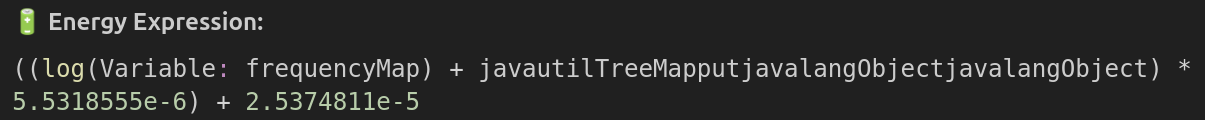
\includegraphics[width = .8 \textwidth]{figures/extension_expression_example.png}
  \caption{Expression for method Map.put(Object, Object)}
  \label{fig:extension_expression_example}
\end{figure}


Another useful feature is the line that spends more energy in each method. Being the line a user defined function or a model trained method, the line will appear highlighted, helping the developer in case of needing help on where to start when needing to refactor the code for energy efficiency. The example can be seen in the Figure~\ref{fig:most_expensive_line}.

\begin{figure}[htbp]
  \centering
  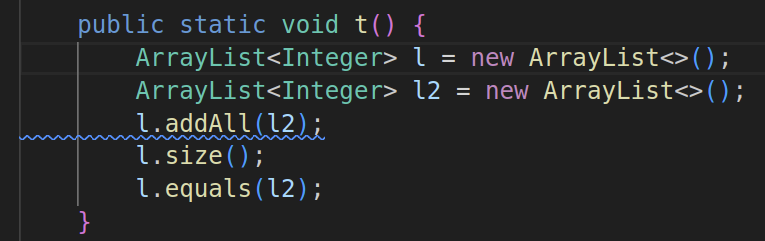
\includegraphics[width = .6 \textwidth]{figures/most_expensive_line.png}
  \caption{Most expensive line highlighted}
  \label{fig:most_expensive_line}
\end{figure}

The extension can be open in a Java project and gather the total energy used by the user made methods, allowing for a better understanding of the code energy impact. Naturally, the extension is limited by the set of pre-trained models it relies on. If a program uses methods that aren't covered by these models, the extension will report an energy usage of zero, which is inaccurate, as those methods still consume energy.

This highlights the importance of continuously expanding the set of pre-trained models to cover a wider range of methods and scenarios. As more energy profiles are collected, the models will be able to predict more accurately the energy consumption of the code.

The extension is designed to be extensible, allowing for the addition of more energy profiles, features,  and models as they become available. This ensures that the entire framework remains relevant and useful for developers as they work on increasingly complex projects.